% main.tex
% Universitaire Papers - Full Documentation & Usage Guide
% Author: Matt
% Purpose: A self-contained manual that explains paperSettings.tex,
%          standardCommands.tex and demonstrates how to use the macros.
%
% Save this file as main.tex in the root of the repo alongside:
%   - paperSettings.tex
%   - standardCommands.tex
%   - main.bib
%
% Compile with: buildLatexDocument.sh (or fullBuild.sh)
% Or upload to Overleaf and compile there.
% -----------------------------------------

% ----------- Document settings -----------
\documentclass[nonacm, sigconf, balance=true]{acmart}
\include{core/paperSettings} % import custom general paper settings
\include{core/standardCommands} % import custom commands and packages
% -----------------------------------------
\begin{document}

    \begin{SimpleTable}[s{1}s{.3}s{.3}]{}{}
        \TableHeader{TERM & LATEX & LATEX COMMAND}
        \TableRow{1. there exists at least one & \exists & \verb|\exists|}
        \TableRow{2. there exists one and only one & \exists! & \verb|\exists!|}
        \TableRow{3. there is no & \nexists & \verb|\nexists|}
        \TableRow{4. for all & \forall & \verb|\forall|}
        \TableRow{5. not (logical not) & \neg & \verb|\neg|}
        \TableRow{6. or (logical or) & \lor & \verb|\lor|}
        \TableRow{7. division & \div & \verb|\div|}
        \TableRow{8. and (logical and) & \land & \verb|\land|}
        \TableRow{9. implies & \implies & \verb|\implies|}
        \TableRow{10. right implication & \Rightarrow & \verb|\Rightarrow|}
        \TableRow{11. is implied by (only if) & \Longleftarrow & \verb|\Longleftarrow|}
        \TableRow{12. left implication & \Leftarrow & \verb|\Leftarrow|}
        \TableRow{13. if and only if, iff & \iff & \verb|\iff|}
        \TableRow{14. equivalence & \Leftrightarrow & \verb|\Leftrightarrow|}
        \TableRow{15.Subset & \subset & \verb|\subset|}
        \TableRow{16. Logical XOR (exclusive or) & \oplus & \verb|\oplus|}
        \TableRow{17. Union of sets & \cup & \verb|\cup|}
        \TableRow{18. Empty set & \emptyset & \verb|\emptyset|}
        \TableRow{19. Intersection of sets & \cap & \verb|\cap|}
    \end{SimpleTable}

    \clearpage
    \onecolumn


    \section{Propositielogica}
    Propositielogica is de studie van bewijzen. Een propositie is te beantwoorden met waar of niet waar
    Een propositie is $3 < 17$, dit kan je checken op waarheid. Een propositie is $x \implies y$

    \subsection{Proposities}
    We gebruiken in logica variabelen zoals P en Q, dit zijn \textit{atomisch} proposities, deze zijn altijd geschreven in HOOFDLETTERS.
    Deze zijn niet verder op te delen, dus niet opgebouwd van kleinere delen zoals implicaties etc. deze waardes zijn Waar/True/1 of Onwaar/False/0.

    Je hebt ook kleine letters p, q, \ldots, dit zijn niet-atomische proposities, het zijn geen propositionele formules, maar eerder \textit{metavariabelen}.

    \begin{multicols}{2}

        Elke propositionele formule bestaat uit:
        \begin{itemize}
            \item Atomitsche proposities (P, Q, R, \ldots)
            \item true, (T, Waar, 1)
            \item false, (F, Onwaar, 0)
        \end{itemize}

        Deze kunnen ook kleiner opgedeeld zijn, dan zijn dit ook propositionele formules:
        \begin{itemize}
            \item $P \implies Q$ - \textbf{implicatie} als P, dan Q
            \item $P \land Q$ - \textbf{conjunctie} P én Q
            \item $P \lor Q$ - \textbf{disjunctie} P of Q
            \item $\neg P$ - \textbf{negatie} (niet P / P houd geen stand)
        \end{itemize}

    \end{multicols}

    Zoals in de wiskunde ook is heeft propositielogica óók een volgorde, deze is:
    \begin{enumerate}
        \item Haakjes ()
        \item Negatie $\neg$
        \item Conjunctie $\land$
        \item Disjunctie $\lor$
        \item Implicatie $\implies$
    \end{enumerate}

    $\neg P \lor Q \implies Q \land P$ moet gelezen worden als $((\neg P) \lor Q) \implies (Q \land P)$

    Om dit te onthouden kan je deze zij onthouden: ``Hoe Navigeert Connie De Ijssel''

    \subsection{Semantiek van propositie operatoren}

    \begin{SimpleTable}[s{.3}s{.3}s{.3}s{.3}s{.3}s{.3}s{.3}s{.3}s{.3}]{Truthtable van basisoperaties}{}
        \TableHeader{$P$ & $Q$ & $\neg P$ & $P \land Q$ & $P \lor Q$ & $P \oplus Q$ & $P \implies Q$ & $P \equiv Q$}
        \TableRow{0 & 0 & 1 & 0 & 0 & 0 & 1 & 1}
        \TableRow{0 & 1 &   & 0 & 1 & 1 & 1 & 0}
        \TableRow{1 & 0 & 0 & 0 & 1 & 1 & 0 & 0}
        \TableRow{1 & 1 &   & 1 & 1 & 0 & 1 & 1}
    \end{SimpleTable}

    Maar stel, je wilt iets moeilijks bewijzen zoals $\neg P \lor Q \implies Q \land P$, dan kan je dat op de volgende manier doen:

    \vsmall

    \begin{SimpleTable}[s{.3}s{.3}s{.3}s{.3}s{.3}s{.3}]{Truthtable van moeilijkere propositie formule}{}
        \TableHeader{$P$ & $Q$ & $\neg P$ & $\neg P \lor Q$ & $ Q \land P$ &  $\neg P \lor Q \implies Q \land P$}
        \TableRow{0 & 0 & 1 & 1 & 0 & 0}
        \TableRow{0 & 1 & 1 & 1 & 0 & 0}
        \TableRow{1 & 0 & 0 & 0 & 0 & 1}
        \TableRow{1 & 1 & 0 & 1 & 1 & 1}
    \end{SimpleTable}

    Je kan ook met verschillende kleuren pennen een kleine thruthtable schrijven, maar dit is een hele nette manier om het ook te doen.

    \subsection{Voorbij thruth tables}
    Je kan d.m.v een truth table bewijzen of een formule wel of niet houd, maar dat kan ook anders, bijvoorbeeld door het versimpelen van de formules.

    \begin{SimpleTable}[s{.1}s{.5}s{.4}]{}{}
        \TableHeader{ & Expression & Law}
        \TableRow{                  & $(p \implies q) \lor (q \implies p)$      & original}
        \TableRow{$\Leftrightarrow$ & $(\neg p \lor q) \lor (\neg q \lor p)$    & implication}
        \TableRow{$\Leftrightarrow$ & $\neg p \lor ((q \lor \neg q) \lor p)$    & associativity / rearrangement}
        \TableRow{$\Leftrightarrow$ & $\neg p \lor (T \lor p)$                  & tertium non datur}
        \TableRow{$\Leftrightarrow$ & $\neg p \lor T$                           & absorbing property of \(T\)}
        \TableRow{$\Leftrightarrow$ & $T$                                       & absorbing property of \(T\)}
    \end{SimpleTable}

    Deze afleiding kan je maken door de regels te gebruiken die hieronder stan geschreven (er zijn er nog meer).

    \begin{multicols}{3}

        Commutativity:
        \begin{itemize}
            \item $p \land q \Leftrightarrow q \land p$
            \item $p \lor q \Leftrightarrow q \lor p$
        \end{itemize}

        Associativity:
        \begin{itemize}
            \item $p \land (q \land r) \Leftrightarrow (p \land q) \land r$
            \item $p \lor (q \lor r) \Leftrightarrow (p \lor q) \lor r$
        \end{itemize}

        Tertium non datur:
        \begin{itemize}
            \item $p \lor \neg p \Leftrightarrow T$
        \end{itemize}

        Idempotence:
        \begin{itemize}
            \item $p \land p \Leftrightarrow p$
            \item $p \lor p \Leftrightarrow p$
        \end{itemize}

        De Morgan:
        \begin{itemize}
            \item $\neg (p \lor q) \Leftrightarrow \neg p \land \neg q$
            \item $\neg (p \land q) \Leftrightarrow \neg p \lor \neg q$
        \end{itemize}

        Double negation (niet niet is wel):
        \begin{itemize}
            \item $p \Leftrightarrow \neg(\neg p)$
        \end{itemize}

        Properties of T en F:
        \begin{itemize}
            \item $p \lor F \Leftrightarrow p$
            \item $p \land F \Leftrightarrow F$
            \item $q \lor T \Leftrightarrow T$
            \item $q \land T \Leftrightarrow q$
        \end{itemize}

        Implication:
        \begin{itemize}
            \item $(p \implies q) \Leftrightarrow (\neg p \lor q)$
        \end{itemize}

        Contraposition:
        \begin{itemize}
            \item $(p \implies q) \Leftrightarrow (\neg q \implies \neg p)$
        \end{itemize}

    \end{multicols}


    \section{sets}
    Propositielogica heeft ook een manier om over een groep dingen te redeneren, \textit{\textbf{sets}}.
    Deze schrijf tussen accolades met comma's tussen de items: $\{ false, true \}$, $\{ 3, 7, 14 \}$, $\{ red, blue, yellow\}$.
    Dit kan voor kleine sets met de hand, maar als je grote sets wilt schrijven, dan kost dat heel veel tijd, daarom kan je ook: ${ 1, 3, 5, ..., 99}$ om alle oneven cijfers van 1 t/m 99 als set te hebben.
    Of als ${1, 2, 3, ...}$ om alle cijfers vanaf 1 te hebben (oneindig).
    De lengte van een sets is op te schrijven door |A| of #A, waar A een set is met een lengte, de \textbf{cardinality} hier tel je alleen het aantal unieke elementen.
    Als er maar 1 element in een set zit, dan heet dat een \textbf{singleton}.

    Ook kan je de \textit{\textbf{set-builder notation}} gebruiken, hierbij schrijf je het soort element dat je wilt en wat het element kan zijn:
    $\{\text{x : x has the property P}\}$

    \begin{voorbeeld}{Set-builder notation}
        Een collectie van alle prime numbers: $\{\text{x : x is een priemgetal}\}$\\
        Of $\{\text{s : s is een strand in Nederland}\}$.
    \end{voorbeeld}

    Er zijn ook een paar basis sets, die al van tevoren zijn gedefinieerd:

    \begin{itemize}
        \item $\emptyset = \{ \}$ & (the empty set)
        \item $\mathbb{B} = \{ 0, 1 \} $ & (the binaire set)
        \item $\mathbb{N} = \{ 0, 1, 2, 3, ... \}$ & (De natuurlijke nummers)
        \item $\mathbb{Z} = \{ ..., -2, -1, 0, 1, 2, ... \}$ & (De integers)
        \item $\mathbb{Q} = \{\dfrac{m}{n} : \text{m, n} \in \mathbb{Z} \text{, n} \neq \text{0} \}$ & (De rationele nummers)
        \item $\mathbb{R} =  \{ x : \text{x is a real number} \}$ & (De real nummers)
    \end{itemize}

    \textbf{$\emptyset$ en \{ $\emptyset$ \} zijn twee verschillende dingen, de een is namelijk: \{ \}, terwijl de ander \{ \{ \} \} is!}

    \subsection{leden en gelijkheid}
    Je kan bekijken of een set een bepaalde member heeft door $7 \in \{3,7,14\}$ te doen.
    Hier is $\in$ te lezen als \textit{"is element onderdeel van"}
    Je hebt ook de negatie vorm, $\not\in$, wat \textit{"is element niet onderdeel van"}, oftwel $6 \not\in \{3,7,14\}$ betekend.

    Ook is goed om te weten dat gelijkheid op basis van unieke element rust, dus $\{1, 2, 3, 2, 1\} \eq \{1, 3, 2\}$.
    Ongelijkheid is dus te bepalen door te kijken of een van de twee sets een waarde heeft die niet in de ander voorkomt.
    Dus volgorde maakt niet uit, en hoeveelheid elementen die dan welniet hetzelfde zijn maakt ook niet uit.

    \subsection{subsets and supersets}
    Een \textit{\textbf{subset}} is een set waarin minstens een deel van de waardes van de superset in voorkomen.

    \begin{multicols}{2}
        Dus $A = \{1, 2, 3\}$ is een subset van $B = \{1, 2, 3, 4\}$, hierin is B een \textit{\textbf{superset}} van A en A een \textit{\textbf{subset}} van B
        Dit schrijf je als volgt: $A \subseteq B$ \textit{(A is included or contained in B)} en vice versa $B \supseteq A$ \textit{(B includes or contains A)}.

        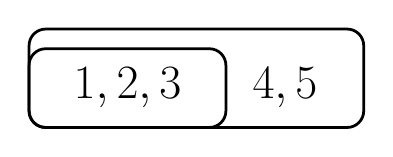
\begin{tikzpicture}
            \tikzstyle{every node}=[font=\LARGE]
            \draw [ line width=1pt , rounded corners = 6.0] (3,9) rectangle (7.25,7.75);
            \draw [ line width=1pt , rounded corners = 6.0] (3,8.75) rectangle (5.5,7.75);
            \node [font=\LARGE] at (4.25,8.25) {$1, 2, 3$};
            \node [font=\LARGE] at (6.25,8.25) {$4, 5$};
        \end{tikzpicture}

    \end{multicols}

    \subsection{Operaties op sets}
    Union $A \cup B = \{x : x \in A \lor x \in B \}$ Combineert A en B met elkaar\\
    Intersection $A \cap B = \{x : x \in A \land x \in B\}$ Het deel wat zowel in A als in B zit\\
    Complement $\overline{A} = \{x : x \not\in A\}$, alles wat niet in A zit.\\
    Difference $A\B = \{x: x \in A \land X \not\in B\}$ Alles wat in A zit, maar niet in B\\

    Zo heb je ook de \textit{powerset P(A)}, dit is een set waarin alle mogelijke subsets van A zitten: $P(A) = \{ X : X \subseteq A \}$.
    Deze heeft $n^2$ elementen, waar n het aantal elementen van set A is.

    \begin{voorbeeld}{powerset/matchsset}
        Stel je hebt een computer scherm, van 1680 x 1050, je wilt elke mogelijke configuratie van zwart/witte pixels opschrijven.
        Een set geeft aan welke pixels wit zijn, dus je wilt elke set met elke mogelijke manier van pixelcoordinaten, dat kan je zo schrijven:

        $W = \{0,1, ..., 1697\}$ voor elke X coordinaat\\
        $H = \{0,1,...,1049\}$ Voor elke Y coordinaat\\
        $W\times H = \{\{0,0\}, \{0,1\}, \{0,2\},...,\{1,0\},...\{1679,1049\}\}$ dit is een volledig wit scherm, elke pixel is gerepresentateerd in deze set\\
        $P(W\times H)$ = elke configuratie van witte pixels
    \end{voorbeeld}

    \subsection{Partities}
    Je kan een set A opdelen in meerdere sets, zoals $A_1$ en $A_2$, hier zijn de regels: $A_1 \cup A_2 = A$ en $A_1 \cap A_2 = \emptyset$
    Zo kan je A = $\mathbb{N}$ opsplitsen in $A_1$ en $A_2$ waar $A_1$ de even getallen zijn en $A_2$ de oneven getallen zijn.

    \subsection{Naive set theory}
    %TODO


    \section{Boolean algebra}
    korte notitie* in Bolean algebra is de $+$ hetzelfde als de OR operator, $\cdot$ hetzelfde als de AND operator, $^{-1}$ hetzelfde als NOT

    \subsection{monoïde}
    Monoide is een verzameling A, is niet ledig en heeft minstens 1 element e, en een binaire operator $\oplus$ %TODO: verder uitschrijven
    Een monoide heeft een nul-element, dit is een waarde die niks doet in de operatie. $x + 0 = x$, hier doet de 0 helemenaal niks, dus 0 is het 0-element in de "+" operatie.
    $x \times 1 = x$, hier is 1 het nul-element in de monoide $\times$ 1; het doet niks in de operatie.
    het is dus een neutrale waarde.

    \subsection{Bool's algebra}

    Boolean algebra heeft een paar regels:

    \begin{itemize}
        \item een set B
        \item Twee elementen $0 \in B$ en $1 \in B$, genaamd \textbf{zero} en \textbf{unit}
        \item Twee binaire operatoren $+$ en $\cdot$ som/OR en product/AND respectievelijk.
        \item Een Unaire operator $^{-1}$ de inverse genoemd ofwel NOT (kan ook als $x'$ zijn genoteerd).
    \end{itemize}

    \begin{voorbeeld}{Bewijs dat $x + x = x$}
        We willen bewijzen dat voor elke $x, x + x = x$\\
        \begin{SimpleTable}[s{.3}s{1}s{.3}]{}{}
            \TableRow{$x + x$ & $= (x + x) \cdot 1$               & Ident}
            \TableRow{        & $= (x + x)\cdot (x \cdot x^{-1})$ & Complement}
            \TableRow{        & $= x + (x \cdot x^{-1})$          & Distrobution}
            \TableRow{        & $= x + ()$                        & Complement}
            \TableRow{        & $= x$                             & Ident}
        \end{SimpleTable}
    \end{voorbeeld}

    \subsection{dualiteit}
    Je kan voor elke vergelijking die je opschrijft een soort duale tweede vergelijking maken door hetvoglende te doen:

    \begin{itemize}
        \item 0 met 1 vervangen
        \item 1 met 0 te vervangen
        \item $+$ met $\cdot$ te vervangen
        \item $\cdot$ met $+$ te vervangen
    \end{itemize}

    \subsection{waarheidstabel naar formule/circuit}
    Stel je krijgt een waarheidstabel zoals deze:

    \begin{multicols}{2}
        \begin{SimpleTable}[s{.3}s{.3}s{.3}]{}{}
            \TableHeader{$x$ & $y$ & $z$}
            \TableRow{0 & 0 & 0}
            \TableRow{0 & 1 & 1}
            \TableRow{1 & 0 & 1}
            \TableRow{1 & 1 & 0}
        \end{SimpleTable}

        Als je dit omzet naar een propositie, dan moet je kijken naar alle rijen waar de uitkomst 1 is.
        Voor elke 0 waarde schrijf je de variabele (hier x of y), op als $\overline{x}\text{ of }\overline{y}$.
        Elke 1 waarde schrijf je alleen de variabele op, dus x of y.
        Als je dat hier zou doen dan krijg je hetvolgende antwoord: $(\overline{x} \land y) \lor (x \land \overline{y})$.
        Dit kan je dan vervolgens omzetten naar een circuit:
    \end{multicols}

    \begin{figure}[h]
        \raggedright
        \includegraphics[width=40mm]{images/boolean_circuit}
    \end{figure}


    \newpage
    \section{Predikatenlogica}

    \subsection{Predicaten en vrije variabelen}

    We zagen eerder de \textit{set-builder}-notatie
    \[
        \{x \mid x \text{ heeft eigenschap } P\},
    \]
    waarbij \(P\) een voorwaarde is. Een voorbeeld van zo’n voorwaarde is
    \[
        P(x) = Prime(x) = \text{``$x$ is een priemgetal''}.
    \]
    Het predicaat geeft voor elke waarde \(x\) waar of onwaar terug, en op basis daarvan bepalen we of \(x\) tot de verzameling behoort. De bijbehorende \textit{truth set} bestaat uit alle waarden die voldoen aan het predicaat.

    \begin{voorbeeld}{Eendjes}
        We hebben zeven eendjes:
        \[
            Eendjes = \{Kwik, Kwek, Kwak, Dagobert, Donald, Katrien, Dumbella\}.
        \]

        We definiëren het predicaat
        \[
            Female(x) = \text{``$x$ is vrouwelijk''}.
        \]

        \begin{itemize}
            \item \(Female(Katrien) \land Female(Dumbella)\) is waar.
            \item \(Female(Kwik) \land Female(Kwek) \land \dots \land Female(Donald)\) is niet waar.
            \item De truth set van \(Female(x)\) is dus \(\{Katrien, Dumbella\}\).
        \end{itemize}
    \end{voorbeeld}

    \subsection{Kwantificatoren en gebonden variabelen}

    Stel dat we willen controleren of elke waarde in een lijst aan een voorwaarde voldoet. Het boek geeft het volgende voorbeeld:

    Er zijn vier kinderen:
    \[
        Kinderen = \{Joel, Felix, Oskar, Amanda\}.
    \]

    Eén van hen moet voorin op de passagiersstoel zitten, omdat er achterin maar drie plekken zijn. Het predicaat \(Front(x)\) betekent dat kind \(x\) voorin zit. We weten dus zeker dat voor één waarde van \(x\) het predicaat waar moet zijn.

    De samengestelde propositie
    \[
        Front(Joel) \lor Front(Felix) \lor Front(Oskar) \lor Front(Amanda)
    \]
    moet waar zijn. Dat levert in principe een grote lijst aan mogelijke combinaties op, wat snel onoverzichtelijk wordt.
    \\
    \\
    Als je een predikaat schrijft zoals $P(x) = \dots x \dots$, dan is x een gebonden variabele.
    Als je een predikaat schrijft zoals $P(x) = \dots y \dots$, dan is y een vrije variabele.\\
    Bij gebonden variabelen kan je de x vervangen door een waarde, $P(x) = x > 1337$. $P(10000)$ wordt dan $10000 > 1337$

    \subsection{Universele kwantificator}

    Om dit compacter te schrijven gebruiken we de universele kwantor \(\forall\).
    De notatie \(\forall x\, P(x)\) betekent: “voor elke \(x\) geldt \(P(x)\)”.
    De propositie is alleen waar wanneer alle waarden voldoen aan \(P\).

    Het voorbeeld
    \[
        Happy(Joel) \land Happy(Felix) \land Happy(Oskar) \land Happy(Amanda)
    \]
    kun je schrijven als
    \[
        \forall x\, Happy(x),
    \]
    waarbij de vraag is: zijn Joel, Felix, Oskar én Amanda allemaal blij?

    \subsection{Existentiële kwantificator}

    Als je wilt uitdrukken dat er minstens één waarde is waarvoor het predicaat waar is, gebruik je de existentiële kwantor \(\exists\).

    De notatie \(\exists x\, P(x)\) betekent: “er bestaat een \(x\) waarvoor \(P(x)\) geldt”.
    Deze propositie is waar wanneer één of meer waarden voldoen aan \(P\).

    Het voorbeeld
    \[
        Happy(Joel) \lor Happy(Felix) \lor Happy(Oskar) \lor Happy(Amanda)
    \]
    kan worden geschreven als
    \[
        \exists x\, Happy(x).
    \]

    Daarnaast bestaat er de vorm \(\exists! x\, P(x)\):
    “Er bestaat precies één \(x\) waarvoor \(P(x)\) geldt.”

    \subsection{Gebonden kwantificatoren}

    Je kunt kwantoren beperken tot een verzameling.

    De universele, beperkte vorm:
    \[
        \forall x \in A\; P(x)
        \quad\text{(alle waarden in \(A\) voldoen aan \(P\)).}
    \]

    De existentiële, beperkte vorm:
    \[
        \exists x \in A\; P(x)
        \quad\text{(er bestaat minstens één waarde in \(A\) die voldoet aan \(P\)).}
    \]

    \subsection{predikatenlogica lezen}

    \begin{itemize}[leftmargin=*]
        \item \( \forall x\,P(x)\) \quad → \quad ``Voor alle \(x\) geldt: \(P(x)\)''. ``Elke \underline{[type van $x$]} heeft de eigenschap ...''.
        \item \( \exists x\,P(x)\) \quad → \quad ``Er bestaat een \(x\) zodanig dat \(P(x)\)''. ``Er is ten minste één \underline{[type]} waarvoor ...''.
        \item \( \exists! x\,P(x)\) \quad → \quad ``Er bestaat precies één \(x\) zodanig dat \(P(x)\)''. In goed Nederlands: ``Er is precies één ... die/het ...''.
        \item \(P(x)\wedge Q(x)\) \quad → \quad ``\(P(x)\) en \(Q(x)\)''.
        \item \(P(x)\vee Q(x)\) \quad → \quad ``\(P(x)\) en/of \(Q(x)\)''.
        \item \(P(x)\rightarrow Q(x)\) \quad → \quad ``Als \(P(x)\), dan \(Q(x)\)''.
        \item \(\neg P(x)\) \quad → \quad ``niet \(P(x)\)''.
        \item \(x = y\) \quad → \quad ``\(x\) en \(y\) zijn hetzelfde object''.
        \item Meerdere kwantoren: volg strikt de volgorde \(\forall x\exists y\) → ``Voor elke \(x\) bestaat een \(y\) ...'', \(\exists y\forall x\) → ``Er bestaat een \(y\) die voor alle \(x\) ...'' (volgorde verandert betekenis!).
    \end{itemize}

    \begin{voorbeeld}{Een Predikatenlogica formule lezen}
    \[
        \forall x\big( Student(x) \to \exists y( Course(y) \land Enrolled(x,y) \land \neg Failed(x,y))\big).
    \]

    \textbf{Stap 1:} Kies domein = ``personen en vakken'': variabele \(x\) = persoon, \(y\) = vak.

    \textbf{Stap 2:}
    \begin{itemize}
        \item Buitenste kwantor: \(\forall x\) — ``Voor alle personen \(x\) geldt: ...''
        \item Binnen: \(Student(x) \to \exists y(\dots)\) — een implicatie: ``als \(x\) student is, dan bestaat er een \(y\) zodanig dat ...''
        \item Binnenste existentie: \(\exists y( Course(y) \land Enrolled(x,y) \land \neg Failed(x,y))\).
    \end{itemize}

    \textbf{Stap 3:}
    \begin{quote}
        Voor elke persoon \(x\): als \(x\) een student is, dan bestaat er een vak \(y\) zodanig dat \(y\) een vak is, \(x\) staat ingeschreven voor \(y\), en het is niet zo dat \(x\) voor \(y\) gezakt is.
    \end{quote}

    \textbf{Stap 4:}
    Herschrijf de zin:
    \begin{quote}
        Elke student is ingeschreven voor minstens één vak waarin die niet gezakt is.
    \end{quote}
    \end{voorbeeld}

    \section{Proof Strategies}

    \begin{multicols}{2}

    \subsection*{Implication ($P \Rightarrow Q$)}

    \noindent\textbf{Introductie (⇒I):}
    Om $P \Rightarrow Q$ te bewijzen neem je $P$ aan en leid je $Q$ af.
    $$
    \text{Assume } P \quad\vdots\quad Q \quad\Rightarrow\quad P \Rightarrow Q
    $$

    \noindent\textbf{Eliminatie (⇒E):}
    Als je zowel $P$ als $P\Rightarrow Q$ hebt, mag je $Q$ concluderen.
    $$
    P,\ \ P\Rightarrow Q \quad\Rightarrow\quad Q
    $$


    \subsection*{Conjunction ($P \land Q$)}

    \noindent\textbf{Introductie (∧I):}
    Bewijs beide delen afzonderlijk.
    $$
    P,\ Q \quad\Rightarrow\quad P \land Q
    $$

    \noindent\textbf{Eliminatie (∧E):}
    Uit $P\land Q$ mag je elk deel los gebruiken.
    $$
    P\land Q \Rightarrow P
    \qquad\qquad
    P\land Q \Rightarrow Q
    $$


    \subsection*{Disjunction ($P \lor Q$)}

    \noindent\textbf{Introductie (∨I):}
    Als één van beide waar is, mag je de disjunctie concluderen.
    $$
    P \Rightarrow P\lor Q
    \qquad\qquad
    Q \Rightarrow P\lor Q
    $$

    \noindent\textbf{Eliminatie (∨E):}
    Als je $P\lor Q$ hebt, bewijs je je doel $R$ in twee gevallen: eerst uit $P$, daarna uit $Q$.
    $$
    \frac{P\lor Q \qquad (P \Rightarrow R) \qquad (Q \Rightarrow R)}{R}
    $$
    Dit is de meest subtiele regel: je moet beide takken afhandelen.


    \subsection*{Negation ($\neg P$)}

    \noindent\textbf{Introductie (¬I):}
    Neem $P$ aan en toon dat dit tot een contradictie leidt.
    $$
    \text{Assume } P \quad\vdots\quad \bot \quad\Rightarrow\quad \neg P
    $$

    \noindent\textbf{Eliminatie (¬E):}
    Uit $P$ en $\neg P$ volgt onmiddellijk een contradictie.
    $$
    P,\ \neg P \quad\Rightarrow\quad \bot
    $$


    \subsection*{Falsity ($\bot$)}

    \noindent\textbf{Eliminatie (⊥E):}
    Uit een contradictie mag je alles afleiden (ex falso).
    $$
    \bot \Rightarrow P
    $$


    \subsection*{Equivalence ($P \Leftrightarrow Q$)}

    \noindent\textbf{Introductie (⇔I):}
    Bewijs beide implicaties.
    $$
    (P \Rightarrow Q) \land (Q \Rightarrow P) \quad\Rightarrow\quad P \Leftrightarrow Q
    $$

    \noindent\textbf{Eliminatie (⇔E):}
    Uit een equivalentie mag je één van de twee implicaties halen.
    $$
    P\Leftrightarrow Q \quad\Rightarrow\quad P\Rightarrow Q
    $$
    $$
    P\Leftrightarrow Q \quad\Rightarrow\quad Q\Rightarrow P
    $$


    \subsection*{Universele kwantor ($\forall x\,P(x)$)}

    \noindent\textbf{Introductie (∀I):}
    Kies een volledig willekeurig element $a$ en bewijs dat $P(a)$ geldt.
    $$
    \text{Let $a$ be arbitrary.}\quad P(a) \Rightarrow \forall x\,P(x)
    $$

    \noindent\textbf{Eliminatie (∀E):}
    Je mag de kwantor instantiëren met een concreet element.
    $$
    \forall x\,P(x) \Rightarrow P(a)
    $$


    \subsection*{Existentiële kwantor ($\exists x\,P(x)$)}

    \noindent\textbf{Introductie (∃I):}
    Geef een concreet voorbeeld $a$ waarvoor $P(a)$ geldt.
    $$
    P(a) \Rightarrow \exists x\,P(x)
    $$

    \noindent\textbf{Eliminatie (∃E):}
    Neem een nieuw element $a$ waarvan je aanneemt dat $P(a)$ waar is, en bewijs met die aanname je doel $R$.
    $$
    \exists x\,P(x),\quad
    \text{Assume } P(a) \ \vdots\ R
    \quad\Rightarrow\quad R
    $$
    \end{multicols}

    \section{functies}
    Als je op elk element in eens set een verandering wilt doorvoeren, dan kan je daar een functie voor gebruiken.
    $f : A \longrightarrow B$ betekend dat je op elke element in $A$ een functie uitvoerd en deze in de set $B$ zet.

    Functies zet elke member in een set om in een output (die dan wel niet altijd gelijk of anders is).

    $A$ noemen we het \textbf{domein}, en $B$ noemen we het \textbf{codomein}.
    Je kan ook meerdere argumenten meegeven: $f : A \times B \times C \longrightarrow D
    De hoeveelheid argumenten noem je de \textbf{ariteit}.

    \subsection{afbeelding en pre-afbeelding}
    de iamge van een set is je begint met een set en die zet je om naar de na-functie set.
    De pre-image is het resultaat en die wil je dan omzetten naar het origineel.

    \subsection{speciale functies}


\end{document}